\documentclass{article}

\usepackage[numbers]{natbib}
\usepackage{neurips_2024}

\usepackage[utf8]{inputenc}
\usepackage[T1]{fontenc}
\usepackage{hyperref}
\usepackage{url}
\usepackage{booktabs}
\usepackage{amsfonts}
\usepackage{nicefrac}
\usepackage{microtype}
\usepackage{xcolor}
\usepackage{graphicx}
\usepackage{float}
\usepackage{caption}

\raggedbottom

\title{Let's Decrypt Dot by Dot: Decoding Hidden Computation in Transformer Language Models}

\author{
  Aryasomayajula Ram Bharadwaj \\
  Independent Researcher \\
  \texttt{ram.bharadwaj.arya@gmail.com}
}

\begin{document}

\maketitle

\begin{abstract}
Recent work has shown that transformer models can perform complex reasoning tasks using Chain-of-Thought (COT) prompting, even when the COT is replaced with hidden characters. This paper investigates methods to decode these hidden computations, focusing on the 3SUM task. We analyze a 34M parameter LLaMA model trained on hidden COT sequences and propose a novel decoding method that successfully recovers the original COT. Our findings provide insights into how transformers encode and process information in hidden COT sequences, offering new perspectives on model interpretability and the nature of computation in language models.
\end{abstract}

\section{Introduction}
Chain-of-Thought (COT) prompting has emerged as a powerful technique for improving the performance of large language models on complex reasoning tasks \cite{wei2022chain}. However, recent work by \cite{pfau2023let} demonstrates that these improvements can be achieved even when the COT is replaced with hidden characters (e.g., "..."), raising intriguing questions about the nature of computation being performed within these models.

This paper builds upon the findings of \cite{pfau2023let}, focusing on the 3SUM task as a case study. We aim to decode the hidden computations embedded within the transformer architecture when trained on hidden COT sequences. Our work provides valuable insights into how these models encode and process information, potentially leading to improved model interpretability and more effective training strategies.

\section{Background}

\subsection{The 3SUM Task}
The 3SUM task involves finding three numbers in a given set that sum to zero. In this experiment, it serves as a proxy for more complex reasoning tasks to study the computational capabilities of transformer models \cite{wei2022chain}. For this experiment, we have used the same data representation method and generating process for 3SUM sequences as in \cite{wei2022chain}.

\subsection{Hidden Chain-of-Thought}
In hidden Chain-of-Thought, intermediate reasoning steps are replaced with hidden characters (e.g., "..."). It has been observed in \cite{pfau2023let} that the models trained on hidden sequences still perform well, suggesting that meaningful computation occurs despite the lack of explicit reasoning steps.

\section{Methodology}
We used a 34M-parameter LLaMA model with 4 layers, 384 hidden dimension, and 6 attention heads \cite{touvron2023llama}, the size of the training and test datasets and all other hyperparameters are kept the same as in the "Let's think dot by dot" paper \cite{pfau2023let}. Our analysis focused on three main areas: Layer-wise Representation Analysis, Token Ranking, and Modified Greedy Decoding Algorithm.

\section{Results and Discussion}

\subsection{Layer-wise Analysis}
Our analysis revealed a gradual evolution of representations across the model's layers. The initial layers primarily contained raw numerical sequences associated with the 3SUM problem's chain of thought. However, starting from the third layer, we noticed the emergence of hidden tokens. As we progressed through subsequent layers, we observed a steady transition from purely numerical sequences to an increasing prevalence of hidden characters.

This pattern suggests that the model develops the ability to utilize hidden tokens as proxies only in its deeper layers, which aligns with intuitive expectations of how neural networks process information. After conducting a comprehensive evaluation across numerous examples, we found that, on average, there is a marked increase in hidden token usage immediately following the second layer. Furthermore, the final layers of the model demonstrate extensive reliance on these hidden tokens.

For this analysis, we employed nostalgebraist's logit lens method \cite{nostalgebraist2020interpreting}.

\begin{figure}[H]
\centering

\includegraphics[width=\textwidth]{hidden_tokens_percentage_by_layer.png}
\caption{Hidden token occurrence percentages in generated sequences across layers}
\label{fig:hidden_token_percentages}
\end{figure}

\subsection{Token Rank Analysis}
The top-ranked token was consistently the hidden character ("."), while lower-ranked tokens revealed the original, non-hidden COT sequences. This supports the hypothesis that the model replaces all computation with hidden tokens on top while keeping the original computation intact underneath. We have provided a sample snapshot of sequences decoded at each layer for both the top (rank-1) and rank-2 tokens in the appendix section.

\subsection{Modified Greedy Decoding Algorithm}
Based on the observations made in the token rank analysis, we implemented a modified greedy autoregressive decoding method. The steps include: performing standard greedy decoding, selecting the second-highest probability token when encountering a hidden token, and continuing this process for the entire sequence. This resulted in a 100\% match in 3SUM task results with and without hidden tokens. To test the effectiveness of this method, we have also compared this with replacing the hidden token with randomly sampled token instead of the next highest (rank-2) token. The percentages of the original and these modified decoding methods are visualized as plots below.

\begin{figure}[H]
\centering
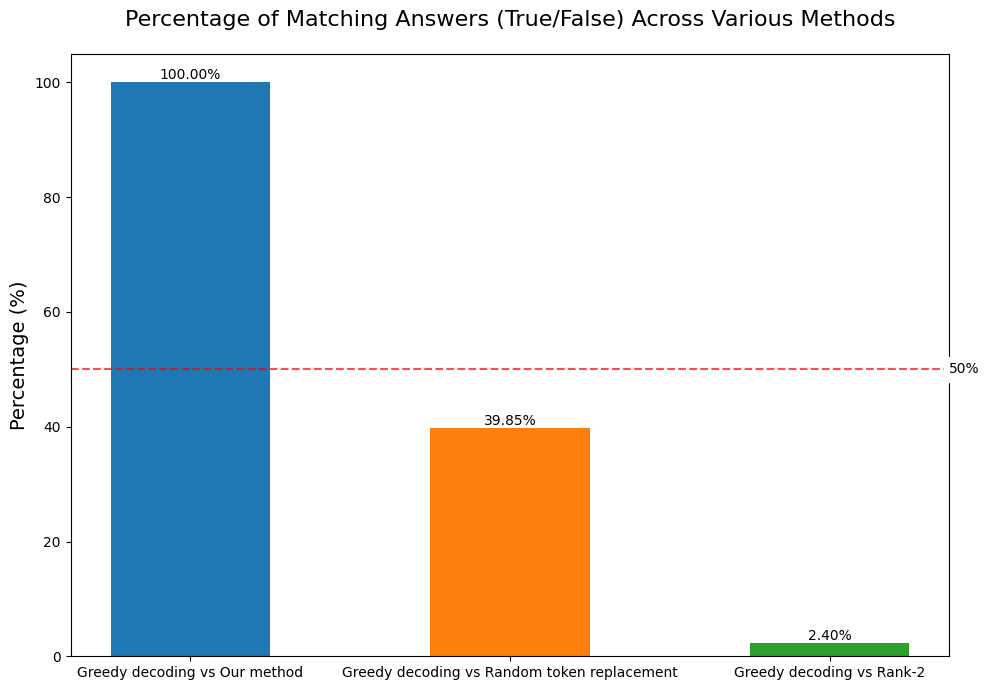
\includegraphics[width=\textwidth]{token_comparison_percentages.png}
\caption{Comparison of decoding methods}
\label{fig:decoding_comparison}
\end{figure}

\section{Implications and Future Work}
Our findings provide new tools for understanding internal reasoning processes and increase confidence in COT-based approaches for improving visibility. Future work should focus on developing better decoding methods or finding circuits that hide tokens, investigating generalizability to tasks beyond 3SUM (including natural language tasks), and improving token hiding methods (currently limited to one hidden token which is simple to decode).

\section{Conclusion}
We have presented a novel approach to understanding hidden computations in transformer models through the analysis of token rankings and layer-wise representations, and the development of a modified decoding algorithm. Our insights into how models encode and process information in hidden COT sequences open new avenues for improving interpretability, efficiency, and safety in language models. This work strengthens the belief in COT visibility research for interpretability.

\section*{Supplemental Materials}
The code to generate the data, train the model and jupyter notebook for analysis performed in the experiments and analysis in this paper is available \href{https://drive.google.com/file/d/1E5ADI6Nc8fm7RQLzV1NkF2YJY1KsngMf/view} here.

\clearpage
\section*{Appendix: Layerwise view of sequences generated via various decoding methods}

\begin{figure}[H]
    \centering
    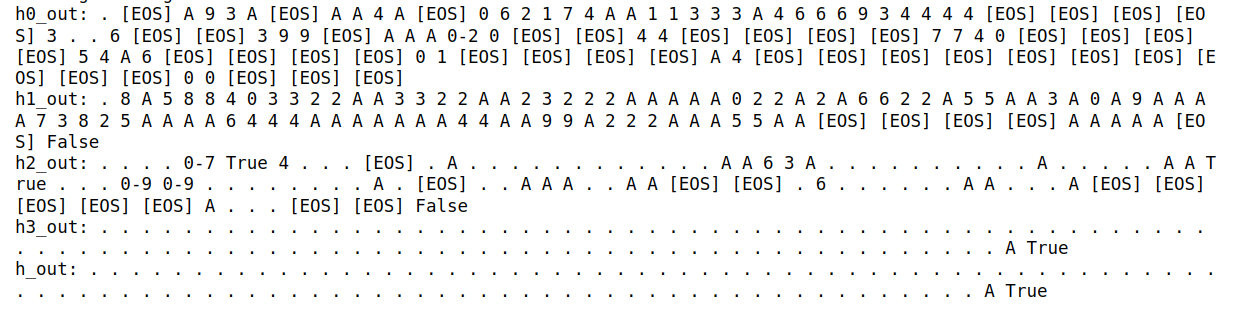
\includegraphics[width=\textwidth]{greedy_decoding.png}
    \caption{Greedy Decoding}
    \label{fig:appendix_greedy}
\end{figure}

\begin{figure}[H]
    \centering
    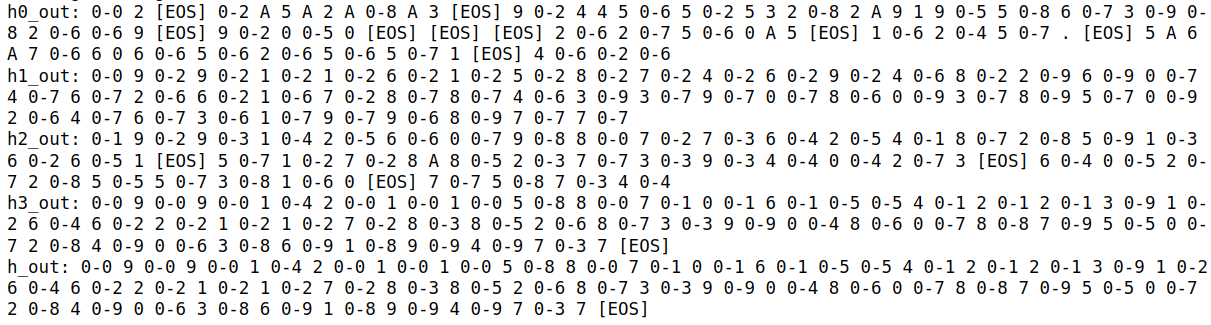
\includegraphics[width=\textwidth]{rank2_decoding.png}
    \caption{Greedy Decoding with Rank-2 Tokens}
    \label{fig:appendix_rank2}
\end{figure}

\begin{figure}[H]
    \centering
    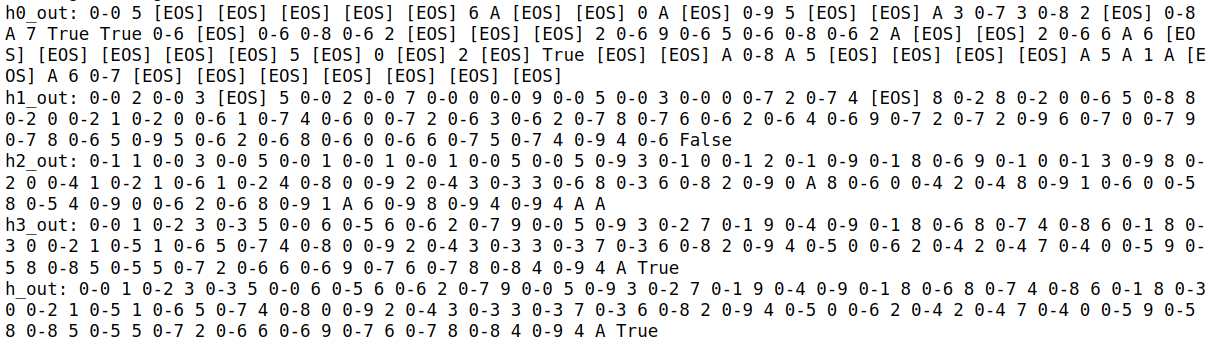
\includegraphics[width=\textwidth]{our_method_decoding.png}
    \caption{Our Method: Greedy Decoding with Hidden Tokens Replaced by Rank-2 Tokens}
    \label{fig:appendix_our_method}
\end{figure}

\begin{figure}[H]
    \centering
    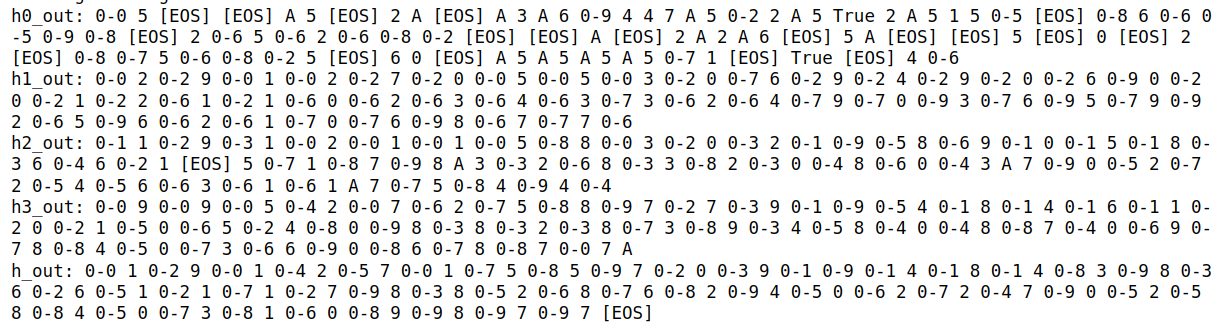
\includegraphics[width=\textwidth]{random_tokens_decoding.png}
    \caption{Greedy Decoding with Hidden Tokens Replaced by Randomly Selected Tokens}
    \label{fig:appendix_random}
\end{figure}

\bibliographystyle{unsrtnat}
\bibliography{references}

\section*{NeurIPS Paper Checklist}

\begin{enumerate}

\item {\bf Claims}
    \item[] Question: Do the main claims made in the abstract and introduction accurately reflect the paper's contributions and scope?
    \item[] Answer: \answerYes{} 
    \item[] Justification: The abstract and introduction clearly state the main contributions of the paper, including the analysis of a 34M parameter LLaMA model, the proposal of a novel decoding method, and insights into how transformers process hidden COT sequences.

\item {\bf Limitations}
    \item[] Question: Does the paper discuss the limitations of the work performed by the authors?
    \item[] Answer: \answerYes{} 
    \item[] Justification: The paper discusses limitations in the "Implications and Future Work" section, mentioning the current limitation to one hidden token and the need for further investigation into generalizability beyond the 3SUM task.

\item {\bf Theory Assumptions and Proofs}
    \item[] Question: For each theoretical result, does the paper provide the full set of assumptions and a complete (and correct) proof?
    \item[] Answer: \answerNA{} 
    \item[] Justification: This paper focuses on empirical analysis and does not present formal theoretical results or proofs.

\item {\bf Experimental Result Reproducibility}
    \item[] Question: Does the paper fully disclose all the information needed to reproduce the main experimental results of the paper to the extent that it affects the main claims and/or conclusions of the paper (regardless of whether the code and data are provided or not)?
    \item[] Answer: \answerYes{} 
    \item[] Justification: The paper provides details on the model architecture, dataset, and methodology used.

\item {\bf Open access to data and code}
    \item[] Question: Does the paper provide open access to the data and code, with sufficient instructions to faithfully reproduce the main experimental results, as described in supplemental material?
    \item[] Answer: \answerYes{} 
    \item[] Justification: While the paper describes the methodology in detail, it does not provide direct access to the code or data used in the experiments.

\item {\bf Experimental Setting/Details}
    \item[] Question: Does the paper specify all the training and test details (e.g., data splits, hyperparameters, how they were chosen, type of optimizer, etc.) necessary to understand the results?
    \item[] Answer: \answerYes{} 
    \item[] Justification: The paper provides details on the model architecture, including the number of layers, hidden dimension, and attention heads. It also mentions that other hyperparameters are kept the same as in the referenced "Let's think dot by dot" paper.

\item {\bf Experiment Statistical Significance}
    \item[] Question: Does the paper report error bars suitably and correctly defined or other appropriate information about the statistical significance of the experiments?
    \item[] Answer: \answerNo{} 
    \item[] Justification: While the paper presents quantitative results, it does not explicitly report error bars or statistical significance tests for the experiments.

\item {\bf Experiments Compute Resources}
    \item[] Question: For each experiment, does the paper provide sufficient information on the computer resources (type of compute workers, memory, time of execution) needed to reproduce the experiments?
    \item[] Answer: \answerNo{} 
    \item[] Justification: The paper does not provide detailed information about the specific compute resources used for the experiments.

\item {\bf Code Of Ethics}
    \item[] Question: Does the research conducted in the paper conform, in every respect, with the NeurIPS Code of Ethics \url{https://neurips.cc/public/EthicsGuidelines}?
    \item[] Answer: \answerYes{} 
    \item[] Justification: The research presented in this paper does not appear to violate any ethical guidelines. It focuses on model interpretability and does not involve sensitive data or potentially harmful applications.

\item {\bf Broader Impacts}
    \item[] Question: Does the paper discuss both potential positive societal impacts and negative societal impacts of the work performed?
    \item[] Answer: \answerNo{} 
    \item[] Justification: While the paper discusses implications and future work, it does not explicitly address potential positive and negative societal impacts of the research.

\item {\bf Safeguards}
    \item[] Question: Does the paper describe safeguards that have been put in place for responsible release of data or models that have a high risk for misuse (e.g., pretrained language models, image generators, or scraped datasets)?
    \item[] Answer: \answerNA{} 
    \item[] Justification: The paper does not involve the release of models or datasets that pose a high risk for misuse.

\item {\bf Licenses for existing assets}
    \item[] Question: Are the creators or original owners of assets (e.g., code, data, models), used in the paper, properly credited and are the license and terms of use explicitly mentioned and properly respected?
    \item[] Answer: \answerYes{} 
    \item[] Justification: The paper cites the original sources for the LLaMA model and the 3SUM task methodology. However, specific license information for these assets is not mentioned in the paper.

\item {\bf New Assets}
    \item[] Question: Are new assets introduced in the paper well documented and is the documentation provided alongside the assets?
    \item[] Answer: \answerYes{} 
    \item[] Justification: The paper introduces a novel decoding method, which is described in detail in the methodology section.

\item {\bf Crowdsourcing and Research with Human Subjects}
    \item[] Question: For crowdsourcing experiments and research with human subjects, does the paper include the full text of instructions given to participants and screenshots, if applicable, as well as details about compensation (if any)? 
    \item[] Answer: \answerNA{} 
    \item[] Justification: This research does not involve crowdsourcing or human subjects.

\item {\bf Institutional Review Board (IRB) Approvals or Equivalent for Research with Human Subjects}
    \item[] Question: Does the paper describe potential risks incurred by study participants, whether such risks were disclosed to the subjects, and whether Institutional Review Board (IRB) approvals (or an equivalent approval/review based on the requirements of your country or institution) were obtained?
    \item[] Answer: \answerNA{} 
    \item[] Justification: This research does not involve human subjects, so IRB approval was not required.

\end{enumerate}

\end{document}
